\documentclass{mcmthesis}
\mcmsetup{CTeX = FALSE,   % 使用 CTeX 套装时,设置为 true
        tcn = 86229, problem = C,
        sheet = true, titleinsheet = true, keywordsinsheet = true,
        titlepage = false, abstract = true}
\usepackage{palatino}
\usepackage{lipsum}
\usepackage{amsmath}
\usepackage{float}

\usepackage{caption}
\usepackage{geometry}
%===============设置正文和数学字体=============================
%有些字体需要安装一些字体文件,注意辨别。
%我参照 MCM论文集的字体 使用如下宏包来定制字体。

\usepackage{graphicx}
\usepackage{subfigure}
%设置段落之间的距离,若不需要删除或者注释掉即可。
\setlength\parskip{.5\baselineskip}
\newtheorem{definition}{Definition}[section]
%\def\abstractname{Summary}%可修改摘要名称

\usepackage{indentfirst}
\setlength{\parindent}{2em}

\usepackage{chngpage}
\usepackage{array}
\usepackage{booktabs}
\usepackage{threeparttable}
\usepackage{longtable}
\usepackage[numbers,sort&compress]{natbib}
%%% 实现参考文献标号在右上角
\newcommand{\upcite}[1]{\textsuperscript{\textsuperscript{\cite{#1}}}}
%然后引用的时候使用\upcite{}的格式(一般的正常引用格式为\cite{})

\usepackage{titletoc}
\titlecontents{section}[3cm]{\bf \large}{\contentslabel{2.8em}}{}{%
\titlerule*[0.5pc]{$\cdot$}\contentspage}%
\titlecontents{subsection}[4cm]{\normalsize}{\contentslabel{2.5em}}{}{%
\titlerule*[0.5pc]{$\cdot$}\contentspage}%
\titlecontents{subsubsection}[5.3cm]{\normalsize}{\contentslabel{3.0em}}{}{%
\titlerule*[0.5pc]{$\cdot$}\contentspage}%

\title{\large \bf{Energy Profile's Description, Forecast and Optimization}}
\author{ }


\date{\today}

\geometry{left=3.0cm,right=3.0cm}

\begin{document}


\begin{abstract}

In the premise of describing, assessing and forecasting the situation of four states (Arizona, California, New Mexico and Texas) energy consumption, after analyzing and examining the condition of population, geography, GDP, policy, externality, contribution to states and industry, we establish a comprehensive model that consists of {\bf{ARIMA model}}, {\bf{AHP model}} as well as {\bf{Logistic and stable model}}.

First of all, we address the energy profile by organizing valid data and presenting it with the chart. Then we formulate {\bf{ARIMA model}} to describe the development of energy consumption for the four states from 1960 to 2009, especially for the cleaner and renewable energy. And then we use it to {\bf{predict}} the energy profile of each state for 2025 and 2050.

Secondly, we consider the mathematical effects of assessing the optimal image of producing and consuming renewable energy and develop a detailed evaluation criterion called {\bf{AHP model}} to quantify the difference. The result is that {\bf{California}} appears to have the best energy profile.

Finally, based on {\bf{AHP model}} as well as {\bf{Logistic and stable model}}, we take three steps to determine renewable energy usage targets for 2025 and 2050. The results show that this four-state energy compact should take actions to adjust the energy allocation immediately. In addition, we conclude a series of {\bf{recommendations}} for the four states to help them meet their energy compact goals. To test how our model works, we perform {\bf{sensitivity analysis}} to our model. It appears that our suggested solution, which is easy to implement and includes detailed assessing model and forecasting model, is broad enough to accommodate various energy consumption conditions.

\begin{keywords}
ARIMA model; AHP model; Logistic and stable model; \\ \hspace*{1.2cm} Cleaner and renewable energy; Interstate cooperation.
\end{keywords}
\end{abstract}

\maketitle
%\pagestyle{empty}
\newpage                                                          %
%==================================================================
%====================生=成=目=录===================================
\begin{adjustwidth}{-1cm}{0cm}

\setcounter{tocdepth}{3}
\thispagestyle{empty}
\tableofcontents                                                  %

\end{adjustwidth}


\newpage

\pagestyle{fancy}

\setcounter{page}{1}
\section{Introduction}
\subsection{Background}

The global energy scene is in a state of flux, with large-scale shifts in the global energy system. These include the rapid deployment and deep declines in the costs of major renewable energy technologies; a growing shift towards electricity in energy use across the globe; profound changes in China's economy and energy policy, moving consumption away from coal; and the continued surge in shale gas and tight oil production in the United States\cite{OECD/IEA}.

A clean energy revolution is taking place across America, underscored by the steady expansion of the U.S. renewable energy sector.

The clean energy industry generates hundreds of billions in economic activity, and is expected to continue to grow rapidly in the coming years. There is tremendous economic opportunity for the countries that invent, manufacture and export clean energy technologies.

The United States decentralizes many aspects of energy policy into state level. There are four states-California (CA), Arizona(AZ), New Mexico (NM), and Texas (TX)-that want to cooperate with each other on the usage of cleaner, renewable energy sources.

\subsection{Problem Restatement}

We are required to provide an energy profile to demonstrate how the four states- CA, AZ, NM and TX-consumed energy from 1960 to 2009. Then we should develop a model to describe concisely the evolution of energy profile for the four states, especially the evolution of cleaner, renewable energy sources. We will interpret our model's result to tell the four governors the similarities and difference about energy profile between the four states. In addition, we should set some criteria to determine which state of the four has the ''best'' profile for use of cleaner, renewable energy in 2009. Under no policy changes by each governor's office, we will predict energy profile of each state for 2025 and 2050.

Using our model for prediction, we will set renewable energy usage targets for 2025 and 2050. To help the four states to accomplish those targets, we will provide some actions that recommended to be carried out.

Finally, based on our analysis of energy profile of the four states and our prediction for renewable energy usage targets, we will make a memo to the group of Governors to help them cooperate with each other to build cleaner circumstances. 

\section{Assumptions}

\begin{itemize}
\item Data is non-stationarity, where an initial differencing step (corresponding to the "integrated" part of the model) can be applied one or more times to eliminate the non-stationarity.
\item The level of using resources reasonably can be described by the conditions of using the cleaner and renewable energy.
 \item The consumption of energy changes ''continuously'', i.e., there will not be some policies that bring sharp changes in energy use.
 \item According to the waste after burning, we assume that the negative externality of natural gas is double than coal and petroleum.
\end{itemize}

\section{List of Notation}

We list the main notations here, and some of the notations will be explained through the modeling process.
\begin{center}
\begin{longtable}{p{.1\textwidth}<{\centering} p{.1\textwidth}<{\centering} 
p{.8\textwidth}m{.4\textwidth}}
\caption{The List of Notation}\\
\toprule[1.5pt]
Number& Symbol& Meaning \\
\midrule

1& $ p $    & Order (number of time lags) of the autoregressive model \\
2& $d$ &    Degree of differencing \\
3& $q$  &  Order of the movingaverage model \\
4& $P$ & Autoregressive terms for the seasonal part of the ARIMA model \\
5& $D$ & Differencing terms for the seasonal part of the ARIMA model \\
6& $Q$ & Moving average terms for the seasonal part of the ARIMA model \\

7& $X_t$      & A time series of data    \\                                                       
8& $t$      & Time  \\
                                                         
9& $L$     & Lag operator                                                     \\
10& $\alpha_i$       & Parameters of the autoregressive part of the model  \\                                         
11& $\theta_i $     & Parameters of the moving average part \\                                                            
12& $\varepsilon _{t}$       & Error terms                             \\

%13& $\rm{CPN}$ & Coal, petroleum and natural gas   \\
%14& $\rm{NCR}$      & Nuclear power and renewable energy \\                                                            

13& $\rm{A}$       & Pair-wise comparison matrix                      \\
14& $w_i$       & Weight of criterion $i$                      \\
15& $n$       & Natural number                       \\
16& $\lambda_{max}$       & Eigenvalue of the matrix \\                                                                
17& $RI$ & Average random consistency index for matrices of order $n$ \\
18& $x_i$ & Rank of the four states, respectively \\
19& $ \rm{C} $ & Improved pair-wise comparison matrix  \\
%22& $ c_{i}$ & Weight of criterion  \\
%23& $ c_i$ & Rank of NM  \\
%24& $ d_i$ & Rank of TX  \\

 \bottomrule[1.5pt]

 \end{longtable}
 \end{center}
\section{Part 1A: Energy Profiles of the Four States}

To create energy profiles for the four states, we divide the energy sources into {\bf{five categories}}: Coal, Petroleum, Natural gas, Nuclear power and Renewable energy. We first address the data provided, i.e., read all the data into MATLAB, omit the repeated data and gather the data that belongs to the same category. Then we plot the energy vs time figure for the four states.

The energy profile for {\bf{Arizona}} is shown in Figure 1. It can be seen that the usage of petroleum increases by year. The consumption of coal also increases but experiences a rapid jump at 1970s. The usage of nuclear experiences a rapid increase at 1980s but also a rapid decrease shortly after. The consumption of natural gas increases, then decreases and increases again. The usage of renewable energy increases steadily, except for 1980s when it experiences a rapid increase and a rapid decrease.

The energy profile for {\bf{California}} is shown in Figure 2. It can be seen that the usage of petroleum, natural gas and renewable energy increases by year. The usage of nuclear power is adopted since 1980s, and increases slowly. California uses coal at a pretty low level, which is environmentally-friend.
 
 \begin{figure}
\begin{minipage}[t]{0.5\linewidth}
\centering
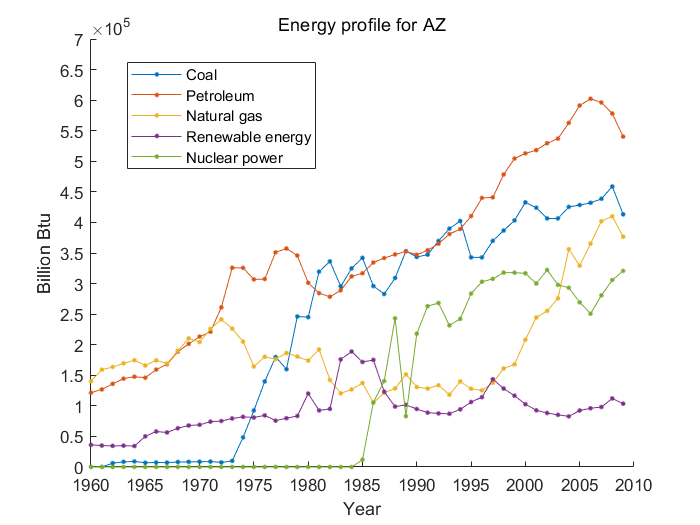
\includegraphics[width=2.8in]{./picture/AZ.png}
\caption{Energy profile for AZ}
\label{fig:left:1}
\end{minipage}%
\begin{minipage}[t]{0.5\linewidth}
\centering
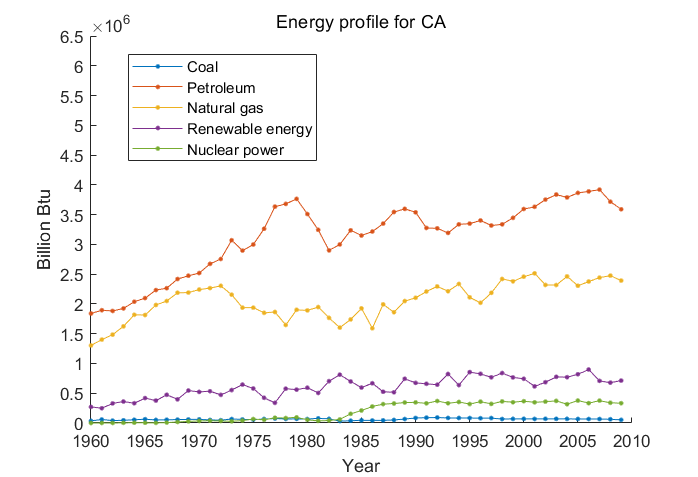
\includegraphics[width=2.9in]{./picture/CA.png}
\caption{Energy profile for CA}
\label{fig:right:1}
\end{minipage}
\end{figure}      
 
The energy profile for {\bf{New Mexico}} is shown in Figure 3. It can be seen that the usage of coal and petroleum increases by year. And the consumption of natural gas experiences an increase, then a decrease and an increase again. The usage of renewable energy is at a low level and increases only for recent years. The consumption of nuclear power is zero from 1960 to 2009.

The energy profile for {\bf{Texas}} is shown in Figure 4. It can be seen that the usage of coal and petroleum increases by year. And the consumption of natural gas experiences an increase, a decrease and then an increase again. The usage of nuclear energy and renewable energy increases slowly.


\begin{figure}
\begin{minipage}[t]{0.5\linewidth}
\centering
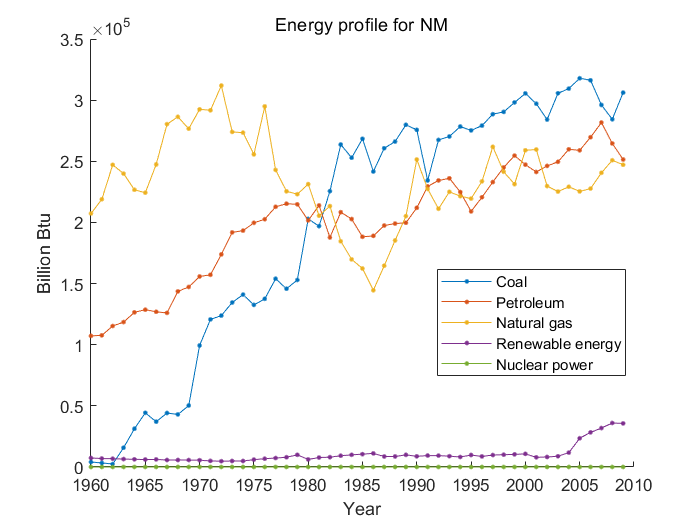
\includegraphics[width=2.9in]{./picture/NM.png}
\caption{Energy profile for NM}
\label{fig:left:2}
\end{minipage}
\begin{minipage}[t]{0.5\linewidth}
\centering
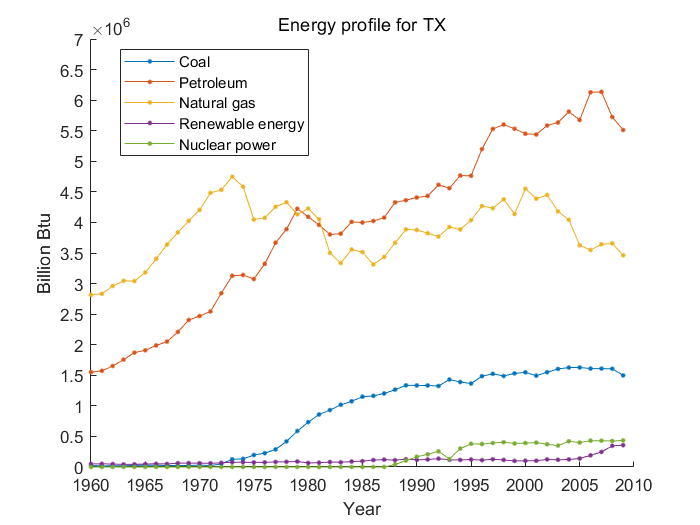
\includegraphics[width=2.8in]{./picture/TX.png}
\caption{Energy profile for TX}
\label{fig:right:2}
\end{minipage}
\end{figure}     

\section{Part 1B: The ARIMA Time Series Model}

\subsection{Model Construction}

In statistics and econometrics, and in particular in time series analysis, an {\bf{autoregressive integrated moving average (ARIMA) model}} is a generalization of an autoregressive moving average (ARMA) model. Both of these models are fitted to time series data either to better understand the data or to predict future points in the series (forecasting). ARIMA models are applied in some cases where data show evidence of non-stationarity, where an initial differencing step (corresponding to the "integrated" part of the model) can be applied one or more times to eliminate the non-stationarity\cite{SAS2015Notation}.

The AR part of ARIMA indicates that the evolving variable of interest is regressed on its own lagged (i.e., prior) values. The MA part indicates that the regression error is actually a linear combination of error terms whose values occurred contemporaneously and at various times in the past. The I (for "integrated") indicates that the data values have been replaced with the difference between their values and the previous values (and this differencing process may have been performed more than once). The purpose of each of these features is to make the model fit the data as well as possible.

Non-seasonal ARIMA models are generally denoted ARIMA$(p,d,q)$ where parameters $p$, $d$, and $q$ are non-negative integers, $p$ is the order (number of time lags) of the autoregressive model, $d$ is the degree of differencing (the number of times the data have had past values subtracted), and $q$ is the order of the moving-average model. 

Seasonal ARIMA models are usually denoted ARIMA$(p,d,q)(P,D,Q)_m$, 
where $m$ refers to the number of periods in each season, and the uppercase $P,D,Q$ refer to the autoregressive, differencing, and moving average terms for the seasonal part of the ARIMA model\cite{Hyndman2015Forecasting, ARIMA}.

Given a time series of data $X_t$ where $t$ is an integer index and the $X_t$ are real numbers, an ARMA$(p',q)$ model is given by

\begin{equation}\label{1}
X_{t}-\alpha _{1}X_{t-1}-\dots -\alpha _{p'}X_{t-p'}=\varepsilon _{t}+\theta _{1}\varepsilon _{t-1}+\cdots +\theta _{q}\varepsilon _{t-q},
\end{equation}

or equivalently by
\begin{equation}\label{2}
{\left(1-\sum _{i=1}^{p'}\alpha _{i}L^{i}\right)X_{t}=\left(1+\sum _{i=1}^{q}\theta _{i}L^{i}\right)\varepsilon _{t},} 
\end{equation}

where $L$ is the lag operator, the $\alpha _{i}$ are the parameters of the autoregressive part of the model, the $\theta _{i}$  are the parameters of the moving average part and the $\varepsilon _{t}$ are error terms. The error terms $\varepsilon _{t}$ are generally assumed to be independent, identically distributed variables sampled from a normal distribution with zero mean.

Assume now that the polynomial $ \textstyle \left(1-\sum _{i=1}^{p'}\alpha _{i}L^{i}\right)$ has a unit root (a factor $(1-L)$ ) of multiplicity $d$. Then it can be rewritten as:

\begin{equation}\label{3}
\left(1-\sum _{i=1}^{p'}\alpha _{i}L^{i}\right)=\left(1-\sum _{i=1}^{p'-d}\phi _{i}L^{i}\right)\left(1-L\right)^{d}.
\end{equation}

An ARIMA$(p,d,q)$ process expresses this polynomial factorisation property with $p=p'-d$, and is given by:

\begin{equation}\label{4}
{\left(1-\sum _{i=1}^{p}\phi _{i}L^{i}\right)(1-L)^{d}X_{t}=\left(1+\sum _{i=1}^{q}\theta _{i}L^{i}\right)\varepsilon _{t},} 
\end{equation}

and thus can be thought as a particular case of an ARMA$(p+d,q)$ process having the autoregressive polynomial with $d$ unit roots. (For this reason, no ARIMA model with $d > 0$ is wide sense stationary.)

The above can be generalized as follows:

\begin{equation}\label{4}
{\left(1-\sum _{i=1}^{p}\phi _{i}L^{i}\right)(1-L)^{d}X_{t}=\delta +\left(1+\sum _{i=1}^{q}\theta _{i}L^{i}\right)\varepsilon _{t}.}
\end{equation}

This defines an ARIMA$(p,d,q)$ process with drift $\delta/\left(1-\sum\phi_i\right)$.

\subsection{Model Results}

Our goal is to describe the evolution of energy sources of the four states from 1960 to 2009. We first divide the energy into {\bf{two classes:}}
 
\begin{itemize}
\item First class (CPN): Coal, petroleum and natural gas;
\item Second class (NCR): clean and renewable energy, including nuclear power and renewable energy.
\end{itemize}

Then we use SPSS software to perform ARIMA model on the addressed data. The SPSS software is able to automatically decide the parameters in ARIMA model, i.e., $p$, $d$ and $q$. In addition, it can fit the data and show the fitting curves.

The results are shown in table 2, where NCRAZ means NCR energy of Arizona, etc. We can know from table 2 what specific ARIMA model the two classes of energy of each states is.

\begin{table}[!ht]
\caption{The ARIMA model of energy evolution}
 \renewcommand\arraystretch{1.5}
 \setlength{\abovecaptionskip}{0pt}%    
\setlength{\belowcaptionskip}{10pt}%
\begin{center}
\begin{tabular}{p{.1\textwidth}p{.19\textwidth}p{.19\textwidth}p{.19\textwidth}p{.18\textwidth}}
\toprule[1.5pt]
Energy & NCRAZ & CPNAZ & NCRCA & CPNCA \\
 \midrule

 Model & ARIMA$(1,1,0)$ & ARIMA$(0,1,0)$ & ARIMA$(1,0,0)$ & ARIMA$(0,1,0)$ \\

 \bottomrule[1.5pt]
 \end{tabular}
 
 \begin{tabular}{p{.1\textwidth}p{.19\textwidth}p{.19\textwidth}p{.19\textwidth}p{.18\textwidth}}
\toprule[1.5pt]
Energy & NCRNM & CPNNM & NCRTX & CPNTX \\
 \midrule

 Model & ARIMA$(0,1,1)$ & ARIMA$(0,1,0)$ & ARIMA$(0,1,0)$ & ARIMA$(0,1,0)$ \\

 \bottomrule[1.5pt]
 \end{tabular}
 
 \end{center} 
 \end{table}

Some of the fitting curves are shown below, including NCR energy evolution for four states, but not all CPN energy. Others will be shown in appendix A.

\begin{figure}[H]
  \centering{
  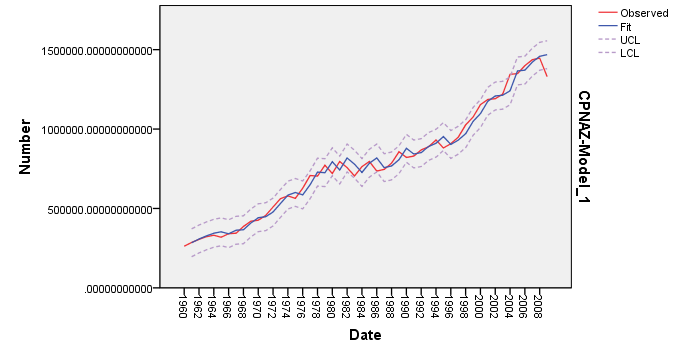
\includegraphics[width=0.8\textwidth]{./picture/CPNAZ.png}}
  \caption{The evolution of CPN energy of AZ}\label{figure5}
\end{figure}

\begin{figure}
\begin{minipage}[t]{0.5\linewidth}
\centering
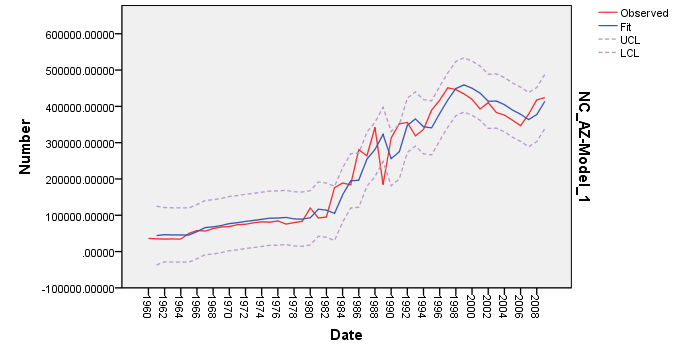
\includegraphics[width=2.9in]{./picture/NCRAZ.png}
\caption{NCR energy's evolution-AZ}
\label{fig:left:3}
\end{minipage}
\begin{minipage}[t]{0.5\linewidth}
\centering
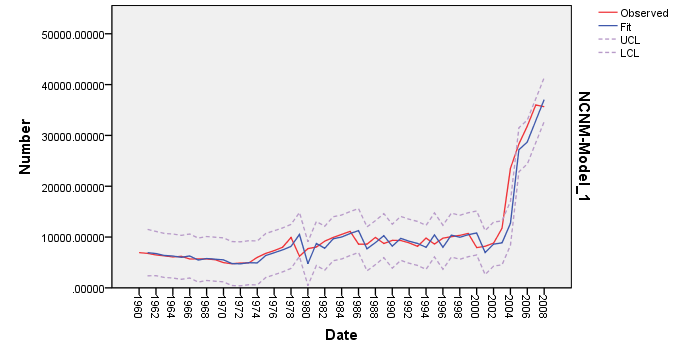
\includegraphics[width=2.9in]{./picture/NCRNM.png}
\caption{NCR energy evolution-NM}
\label{fig:right:3}
\end{minipage}
\end{figure}   

\begin{figure}
\begin{minipage}[t]{0.5\linewidth}
\centering
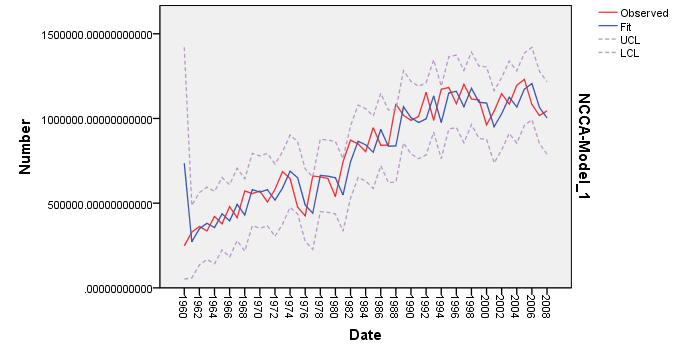
\includegraphics[width=3.0in]{./picture/NCRCA.png}
\caption{NCR energy's evolution-CA}
\label{fig:left:4}
\end{minipage}
\begin{minipage}[t]{0.5\linewidth}
\centering
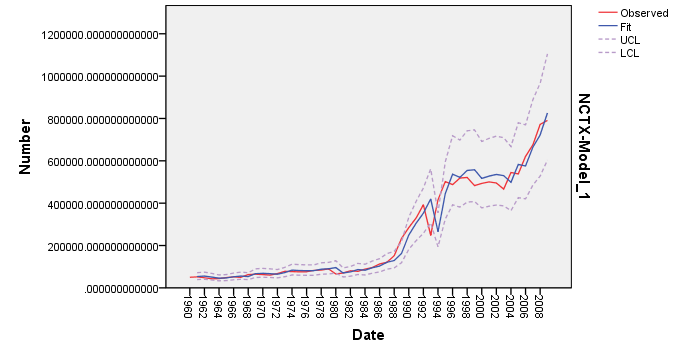
\includegraphics[width=3in]{./picture/NCRTX.png}
\caption{NCR energy evolution-TX}
\label{fig:right:4}
\end{minipage}
\end{figure}  

\subsection{Analysis and interpretation of the model results}

The evolution of {\bf{ nuclear energy}} of the four states is shown in figure 10. Then we can conclude the similarities and difference between the four states.

\begin{figure}[H]
  \centering{
  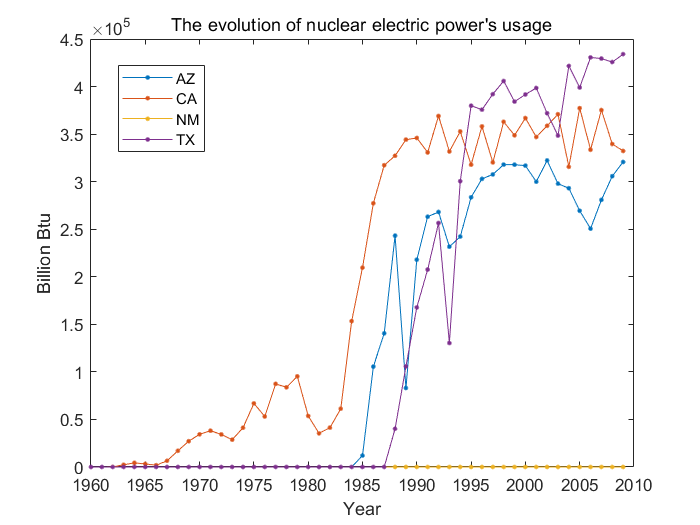
\includegraphics[width=0.7\textwidth]{./pictureb/nuclear.png}}
  \caption{The evolution of nuclear energy}\label{figure10}
\end{figure}

\newpage

{\bf{Similarities:}}

\begin{itemize}
\item The usage of nuclear power experience a rapid increase at 1980s except for New Mexico
\item The amount of nuclear power used is about equal after 1995 for California, Arizonia and Texas.
\end{itemize}

{\bf{Difference:}}

\begin{itemize}
\item California started to use nuclear energy first at 1960s, but Arizonia and Texas began to use at 1980s. New Mexico even never used nuclear power.
\item Texas started using nuclear power late but poduced the highest amount after 1995.
\end{itemize}

The evolution of {\bf{renewable energy}} of the four states is shown in figure 11. We conclude the similarities and difference between the four states as follows:

\begin{figure}[H]
  \centering{
  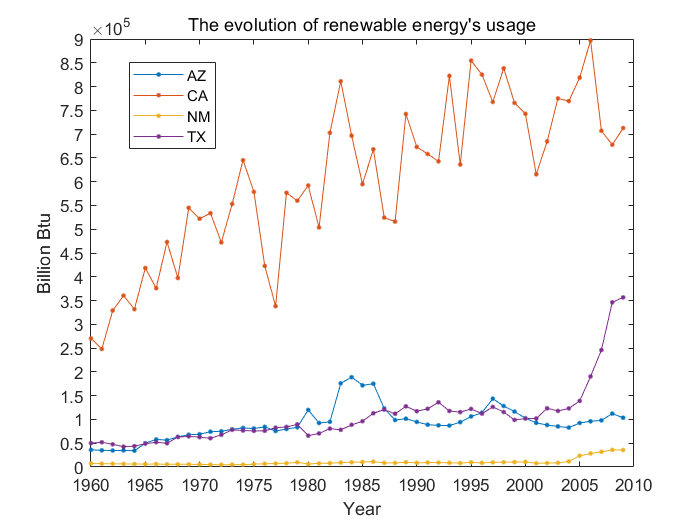
\includegraphics[width=0.7\textwidth]{./pictureb/renewable.png}}
  \caption{The evolution of renewable energy}\label{figure11}
\end{figure}

{\bf{Similarities:}}

\begin{itemize}
\item The amount of renewable energy for Arizona and Texas is nearly the same from 1960 to 2000.
\item The usage of renewable energy roughly increases by year.
\end{itemize}

\newpage

{\bf{Difference:}}

\begin{itemize}
\item California uses renewable energy more than the rest three states, which is about six times the usage in Arizona and Texas.
\item New Mexico's usage of renewable energy is at a pretty low level, which is about zero until 2005.
\end{itemize}

Seperately, we consider the usage of biomass energy, wind energy as well as solar energy. The consumption of {\bf{biomass energy}} is shown in figure 12. Now we analyze the similarities and difference between the four states.

\begin{figure}[H]
  \centering{
  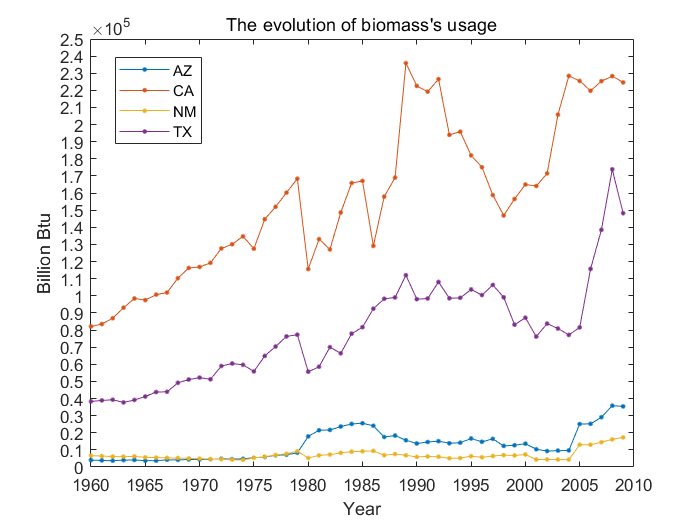
\includegraphics[width=0.7\textwidth]{./pictureb/biomass.png}}
  \caption{The evolution of biomass energy}\label{figure12}
\end{figure}

{\bf{Similarities:}}

\begin{itemize}
\item The usage of biomass energy in California and Texas has the same vibration shape.
\item The usage of biomass energy in New Mexico and Arizona is both at a low level.
\end{itemize}

{\bf{Difference:}}

\begin{itemize}
\item California uses biomass energy more than the rest three states, which is about twice the usage in Texas and far greater than the usage in New Mexico and Arizona.
\item The consumption of biomass energy in California experiences a sharp decrease during 1990s, and a rapid recovery from 1999 to 2004.
\end{itemize}

The consumption of {\bf{wind energy}} is shown in figure 13. We analyze the similarities and difference between the four states as follows:

\begin{figure}[H]
  \centering{
  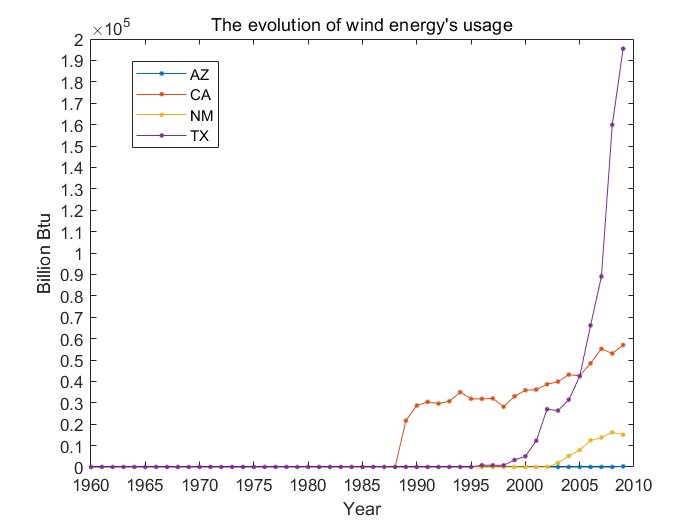
\includegraphics[width=0.7\textwidth]{./pictureb/wind.png}}
  \caption{The evolution of wind energy}\label{figure13}
\end{figure}

{\bf{Similarities:}}

\begin{itemize}
\item The four states didn't use wind energy from 1960 to 1988.
\item The usage of wind energy in California, New Mexico and Arizona increases by year after they started to adopt it.
\end{itemize}

{\bf{Difference:}}

\begin{itemize}
\item The consumption of wind energy in California increased rapidly from 2000 to 2009.
\item Arizona nealy never used wind energy since it didn't have so much wind due to its geography.
\end{itemize}

The consumption of {\bf{solar energy}} is shown in figure 14. Then we can analyze the similarities and difference between the four states.

\begin{figure}[H]
  \centering{
  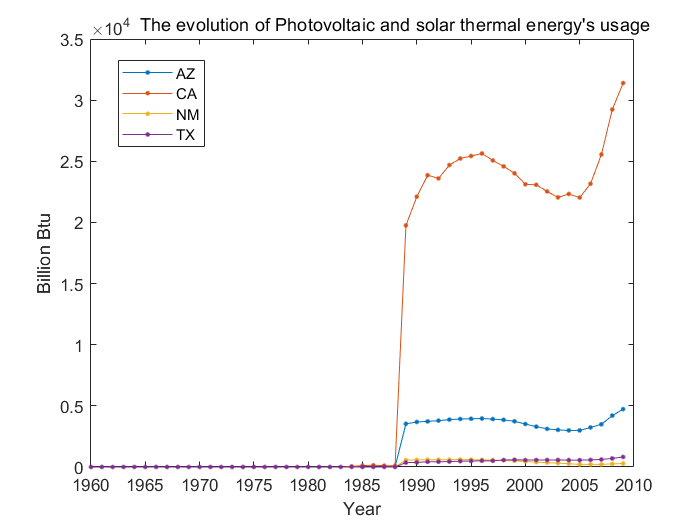
\includegraphics[width=0.7\textwidth]{./pictureb/solar.png}}
  \caption{The evolution of solar energy}\label{figure14}
\end{figure}

{\bf{Similarities:}}

\begin{itemize}
\item The four states didn't use solar energy until 1988, since people find the way to transform solar energy to electricity.
\item After starting to use solar energy, the amount stays stable, since there didn't exist an effective way to increase photoelectric conversion rate.
\end{itemize}

{\bf{Difference:}}

\begin{itemize}
\item California uses solar energy more than the rest three states, which is about five times  the usage in Arizona and far greater than the usage in New Mexico and Texas.
\item The consumption of solar energy in California experiences a decrease from 1995 to 2005, and a rapid recovery from 2005.
\end{itemize}

\subsection{Section Conclusion}

\begin{itemize}
\item The consumption of cleaner and renewable energy in California is always greater than the other three states. The reason is that California has a {\bf{Mediterranean climate}} which is suitable for people to live. With 39.5 million residents, California is the {\bf{most populous}} state. The great amount of population results in huge consumption of all kinds of energy\cite{California}.
\item New Mexico always consumes energy at a relatively low level. The reason is that the New Mexican landscape ranges from wide, rose-colored {\bf{deserts}} to broken mesas to high, snow-capped {\bf{peaks}}. The result is that with a population of approximately two million, New Mexico is the 36th most populous state\cite{NewMexico}. 
\end{itemize}

\section{Part 1C: The Analytic Hierarchy Process Model}

\subsection{Model Construction}

The {\bf{analytic hierarchy process}} (AHP) is a structured technique for organizing and analyzing complex decisions. The AHP consists of the following three steps\cite{Wan2009Application,Carlsson1995AHP}:

\begin{itemize}
\item Step 1: A problem under complicated situations is decomposed into a hierarchy structure. The top-level structure includes a single element which reflects the objective of the AHP analysis. The elements at lower levels are determined objectively by the decision makers according to the relationships between each element at the current level and a certain element at the previous level. Finally, alternative strategies are listed on the lowest level.

\item Step 2: The elements at intermediate levels are weighed. Namely, each element at every level is evaluated about the elements at the previous level to acquire relative weights of the elements at the same level under the criteria.

\item Step 3: The weight of the entire hierarchy is acquired using the weights of the elements at each level. According to the weight, priority of each alternative strategy for the overall objective is acquired.
\end{itemize}

The AHP analysis is based on pair-wise comparison, the scale of the relative importance of a criterion to other criteria established by Saaty (Table 3)\cite{Leung1998Evaluating}. 

\begin{table}[!ht]
\caption{Pair-wise comparison scale for AHP preferences}
 \renewcommand\arraystretch{1.5}
 \setlength{\abovecaptionskip}{0pt}%    
\setlength{\belowcaptionskip}{10pt}%
\begin{center}
\begin{tabular}{p{.3\textwidth}<{\centering} p{.5\textwidth}}
\toprule[1.5pt]
Numerical rating & Verbal judgments of preferences  \\
 \midrule

 9 & Extremely preferred \\
8 & Very strongly to extremely preferred \\
7 & Very strongly preferred \\
6 & Strongly to very strongly preferred \\
5 & Strongly preferred \\
4 & Moderately to strongly preferred \\
3 & Moderately preferred \\
2 & Equally to moderately preferred \\
1 & Equally preferred \\
Reciprocals of above & If factor $i$ has one of the above numbers assigned to it when compared to factor $j$, then $j$ has the reciprocal value when compared with $i$\\

 \bottomrule[1.5pt]
 \end{tabular}
 \end{center} 
 \end{table}

Pair-wise comparison matrix {\bf{A}} is established using the relative importance:

\begin{equation}\label{6}
A=\left[a_{ij}\right], a_{ij}=w_i/w_j, a_{ji}=1/a_{ij}, a_{ii}=1
\end{equation}

Here $w_i$ is the weight of criterion $i$, and $w_j$ is the weight of criterion $j$. The weights from the above matrix can easily be determined by solving the following equation:

\begin{equation}\label{7}
AW=nW, W=\left(w_1,w_2,\dots,w_n\right)^T
\end{equation}

Where $n$ is the natural number or number of decision elements.
From (Eq.(7)), $n$ is determined as eigenvalue $(\lambda_{max})$ of the matrix, that is:

\begin{equation}\label{8}
AW=\lambda_{max}W
\end{equation}

And $w_i$ satisfies the following equation:

\begin{equation}\label{9}
\sum_{i=1}^{n}w_i=1
\end{equation}

The judgment for the satisfaction of $\lambda_{max}$ is made by determining the consistency index and consistency ratio, given by $CI$ and $CR$ from equation (Eq. (10)) and equation (Eq. (11)):

\begin{equation}\label{10}
CI=\left(\lambda_{max}-n\right)/n
\end{equation}

\begin{equation}\label{11}
CR=CI/RI
\end{equation}

$\lambda_{max}$ is the principal eigenvalue of the judgment matrix and $RI$
is the average random consistency index for matrices of order $n$, calculated as follows\cite{Wei2005An}:

\begin{equation}\label{12}
RI=0(n=1,2), 0.58(n=3), 1.12(n=5), 1.24(n=6), 1.32(n=7), 1.41(n=8)
\end{equation}

When $CR$ is greater than 0.10 (10\%), $\lambda_{max}$ is not satisfied,
and inconsistent judgments must be readjusted in order to improve the consistency.

If the sequencing weight vector of the $(k-1)^{th}$ layer factor towards the total goal is $W^{(k-1)}=\left(W_1^{(k-1)}, W_2^{(k-1)},\dots, W_n^{(k-1)}\right)^T$, the entire factors of the $k^{th}$ layer towards the synthetic sequence
vector $W^{(k)}$ of the total goal are given by the following equation (Eq. (13)):

\begin{equation}\label{13}
W^{(k)}=\left(P_1^{(k)},P_2^{(k)},\dots, P_n^{(k)}\right)W^{(k-1)}
=P^{(k)}W^{(k-1)}
\end{equation}

Where $P^{(k)}$($n_k*n_{k-1}$ matrix) is the sequencing weight vector
of the $k^{th}$ layer factor towards the $(k-1)^{th}$ layer factor.

\subsection{Model Results}

We consider six aspects and use letters to represent them, resprectively.

\begin{itemize}
\item 1. The level of using resources reasonably: $x$ 
\item 2. Supporting policy: $y$
\item 3. Contributing to nation energy condition: $z$
\item 4. Negative externality: $M$
\item 5. The degree of clear energy contributing to GDP: $ N$
\item 6. The percentage of clear energy : $K$
\end{itemize}

We use the method of AHP model to rank the four states. On the basis of the data of each above energy production, we rank the four states:

\begin{equation}\label{14}
AZ: a_1, CA: b_1, NM: c_1, TX: d_1.
\end{equation}

Then according to the profile of four states and the estimating storage content of each above energy, we rank the four states as:

\begin{equation}\label{15}
AZ: a_2, CA: b_2, NM: c_2, TX: d_2.
\end{equation}

 To meet the need of describing the level, we set
 
 \begin{equation}\label{16}
AZ: a_2-a_1, CA: b_2-b_1, NM: c_2-c_1 , TX: d_2-d_1.
\end{equation}

 The rest can be done by the same manner:
\begin{align}
AM: x_1=(a_2-a_1)+\dots+(a_{12}-a_{11})\\
CA: x_2=(b_2-b_1)+\dots+(b_{12}-b_{11})\\
NM: x_3=(c_2-c_1)+\dots+(c_{12}-c_{11})\\
TX: x_4=(d_2-d_1)+\dots+(d_{12}-d_{11})
\end{align}

The pair-wise comparison matrix {\bf{A}} is:

\begin{equation}\label{21}
\rm {A}=
\left[ \begin{array}{cccc}
   1 & x_1/x_2 & x_1/x_3 & x_1/x_4 \\
   x_2/x_1 & 1 & x_2/x_3 & x_2/x_4 \\
   x_3/x_1 & x_3/x_2 & 1 & x_3/x_4 \\
   x_4/x_1 & x_4/x_2 & x_4/x_3 & 1
  \end{array}
  \right]
\end{equation}

Analyzing the profile of four states, we describe the degree of supporting policy for our model. We use the divisor of describing the supporting level of policy. We adjust divisor according to different states policy conditions. Initially, the coefficients of four states are all zero. Each reasonable policy of supporting clean energy will add numerical value to divisors.
\begin{align}
&& Z&=\text{clean energy usage}+(\text{total energy production}- \text{total energy usage}) \\
&& M&=-\text{coal usage}\times 2-\text{petroleum usage}\times 2-\text{natural gas usage}\times 1 \\
&& N&=\text{clean energy}/\text{GDP}(2009) \\
&& K&=\text{clean energy}/\text{total energy consumption}
\end{align}

Then we use {\bf{AHP model}} to rank the four states with respect to six aspects defined above\cite{Al2001Application}. The result is shown in table 4.

\begin{table}[!ht]
\caption{The rank results for four states}
 \renewcommand\arraystretch{1.5}
 \setlength{\abovecaptionskip}{0pt}%    
\setlength{\belowcaptionskip}{10pt}%
\begin{center}
\begin{tabular}{p{.3\textwidth}<{\centering} p{.3\textwidth}<{\centering}
p{.3\textwidth}<{\centering} }
\toprule[1.5pt]
States & Grades & Rank  \\
 \midrule

Arizona & 0.557734 & 2 \\
California & 0.654943 & 1 \\
New Mexico & -0.230951 & 4 \\
Texas & 0.521871 & 3 \\
 \bottomrule[1.5pt]
 \end{tabular}
 \end{center} 
 \end{table}

From table 4 we know that {\bf{California}} appears to have the ''best'' profile for use of cleaner, renewable energy in 2009.

\section{Part 1D: Predict the Energy Profiles}

We use the ARIMA model obtained from Part 1B to forecast the energy profile of each state for 2025 and 2050 in the absence of any policy changes by each governor's
office.

The ARIMA model can be viewed as a "cascade" of two models. The first is non-stationary\cite{Lai2002Group}:

\begin{equation}\label{26}
{ Y_{t}=(1-L)^{d}X_{t},}
 \end{equation}
 
while the second is wide-sense stationary:

\begin{equation}\label{27}
{\left(1-\sum _{i=1}^{p}\phi _{i}L^{i}\right)Y_{t}=\left(1+\sum _{i=1}^{q}\theta _{i}L^{i}\right)\varepsilon _{t}.}
\end{equation}

Now forecasts can be made for the process $Y_{t}$, using a generalization of the method of autoregressive forecasting.

We import the data for prediction into SPSS. The predicted results are shown blew. The following eight pie charts describe the proportion of five categraries of energy defined in Part 1A.

\begin{figure}
\begin{minipage}[t]{0.5\linewidth}
\centering
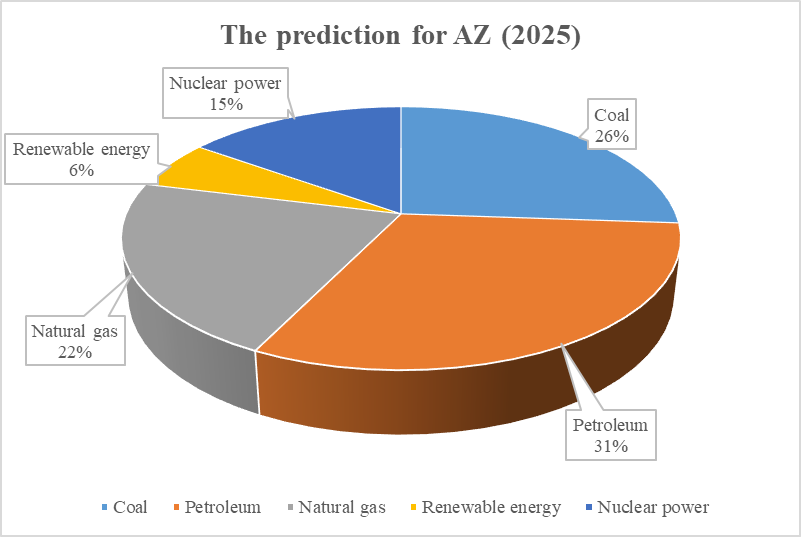
\includegraphics[width=2.6in]{./picturec/AZF2025.png}
\caption{The prediction for AZ (2025)}
\label{fig:left:15}
\end{minipage}%
\begin{minipage}[t]{0.5\linewidth}
\centering
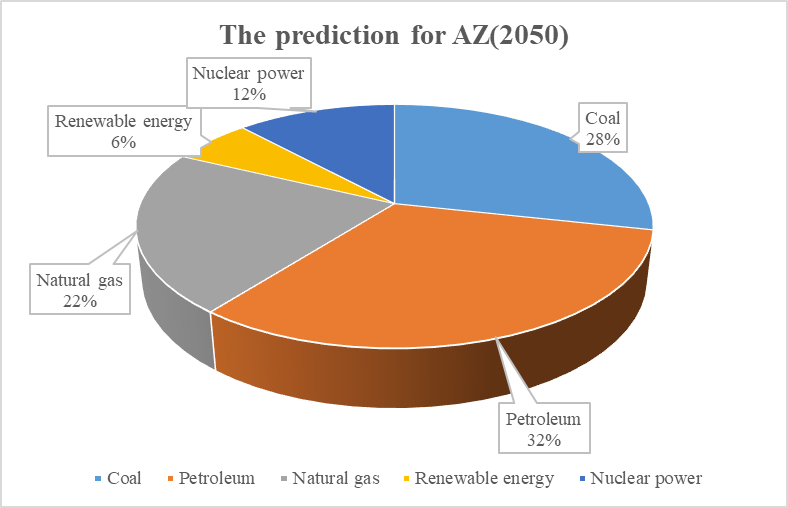
\includegraphics[width=2.7in]{./picturec/AZF2050.png}
\caption{The prediction for AZ (2050)}
\label{fig:right:16}
\end{minipage}
\end{figure}

\begin{figure}
\begin{minipage}[t]{0.5\linewidth}
\centering
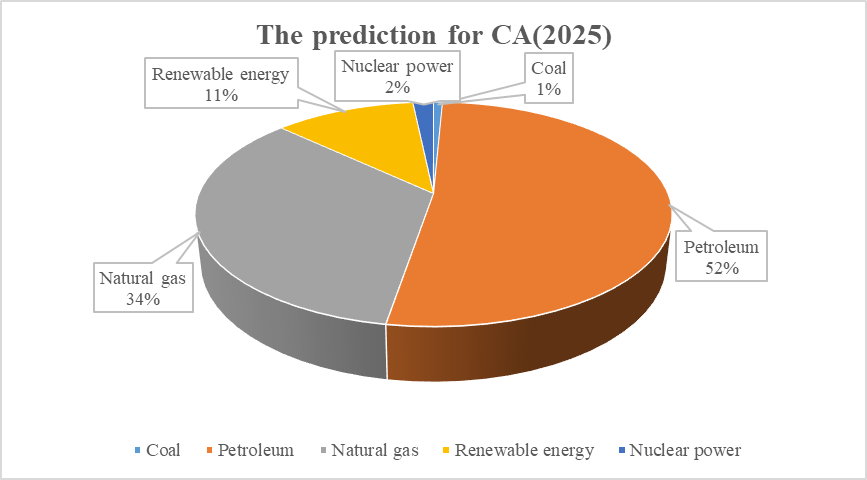
\includegraphics[width=2.8in]{./picturec/CAF2025.png}
\caption{The prediction for CA (2025)}
\label{fig:left:17}
\end{minipage}%
\begin{minipage}[t]{0.5\linewidth}
\centering
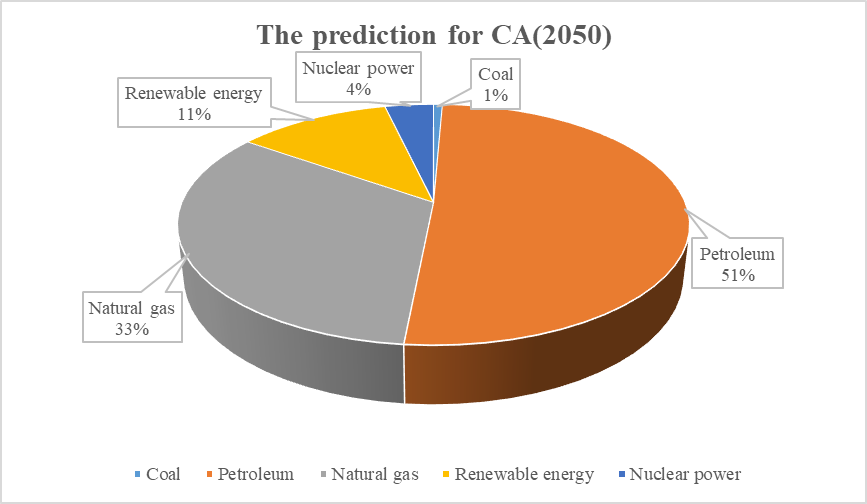
\includegraphics[width=2.7in]{./picturec/CAF2050.png}
\caption{The prediction for CA (2050)}
\label{fig:right:18}
\end{minipage}
\end{figure}                                           

\begin{figure}
\begin{minipage}[t]{0.5\linewidth}
\centering
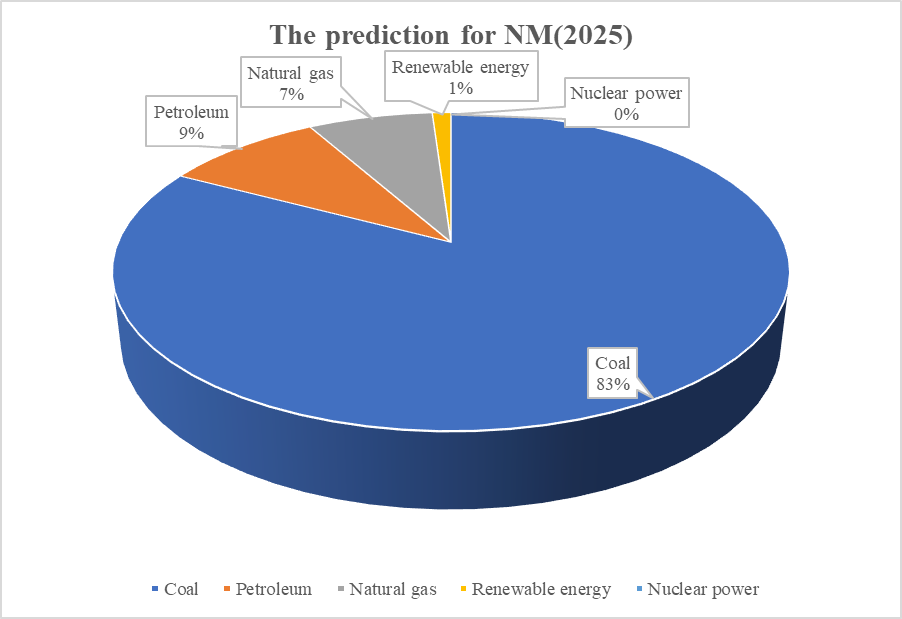
\includegraphics[width=2.6in]{./picturec/NMF2025.png}
\caption{The prediction for NM (2025)}
\label{fig:left:19}
\end{minipage}%
\begin{minipage}[t]{0.5\linewidth}
\centering
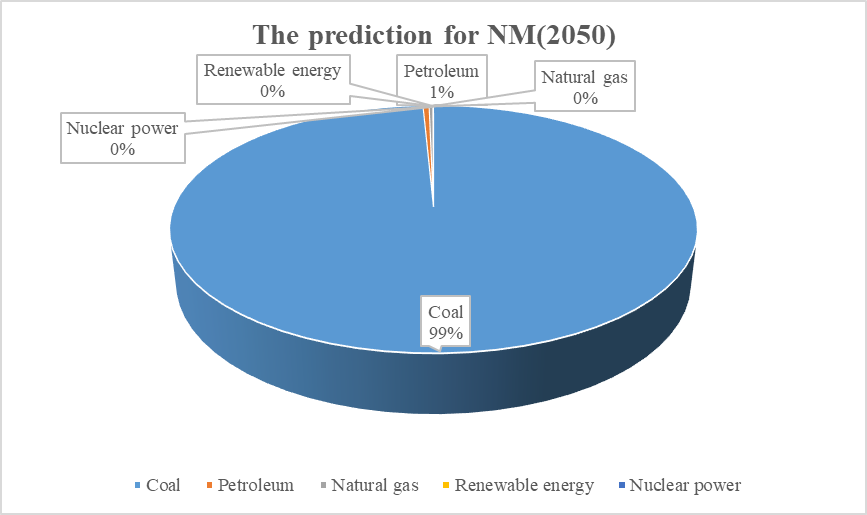
\includegraphics[width=2.95in]{./picturec/NMF2050.png}
\caption{The prediction for NM (2050)}
\label{fig:right:20}
\end{minipage}
\end{figure}     

\begin{figure}
\begin{minipage}[t]{0.5\linewidth}
\centering
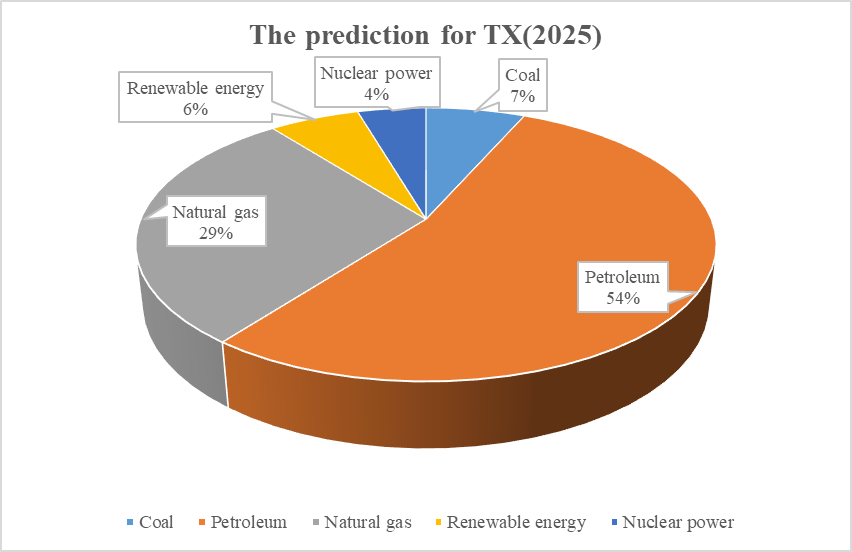
\includegraphics[width=2.9in]{./picturec/TXF2025.png}
\caption{The prediction for TX (2025)}
\label{fig:left:21}
\end{minipage}%
\begin{minipage}[t]{0.5\linewidth}
\centering
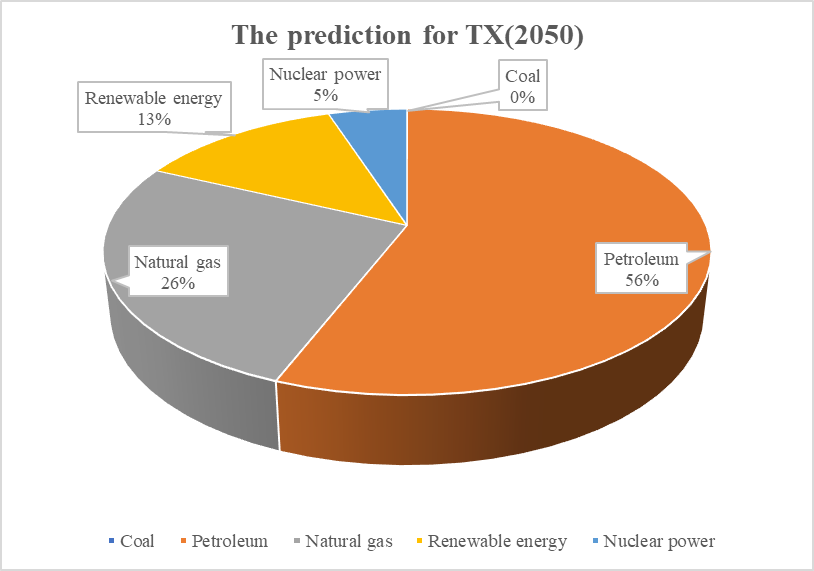
\includegraphics[width=2.7in]{./picturec/TXF2050.png}
\caption{The prediction for TX (2050)}
\label{fig:right:22}
\end{minipage}
\end{figure}     

\section{Part 2A: Renewable Energy Usage Targets}

With the model established in part 1C, we address the problem of optimizing standard of using clear energy. With {\bf{ARIMA model}}, the conditions of using the clear energy in 2025 and 2050 are able to be forecasted. We assume that the forecasted number is $h$. We adjust them by the following methods.

1. We get a pair-wise comparison matrix {\bf{A}} and its eigenvector from part 1C. Take the eigenvector {\bf{B}} corresponding to the maximum eigenvalues:
\begin{align}
&&B&=(r_1, r_2, r_3)^T \\
&&Q&=R_e-R_p \\
&&F&=(a_2-a_1)h\times 9\times \left((r_1+r_2+r_3)/3+1\right)
\end{align}

where $R_e$ is the rank of energy saving condition, $R_p$ is the rank of energy production and $F$ represent the data obtained from the first step.

2. Then we adjust $F$ by analyzing the policy of different states, and other factors such as historical events. For example, California sets a goal to reduce the total energy consumed per dollar of real gross domestic product in half. We use linear regression to forecast the energy condition, and then cut it half. Then we get the second step data.

Based on logistic and stable model, we can obtain the condition of use biomass more realistically.

The main equations of logistic and stable model are:

\begin{equation}
 X(t)=f(x)=r\times x(1-x/N),
\end{equation}

\begin{equation}
C_b=r\times N/4+h,
\end{equation}

where $r$ is  the grouth rate, $N$ is promised by environment biomass, and $C_b$ is the optimal consumption of biomass energy.

The results (renewable energy usage targets) are shown blew in table 5.

\begin{table}[!ht]
\caption{Recommended goals (Billion Btu)}
 \renewcommand\arraystretch{1.5}
 \setlength{\abovecaptionskip}{0pt}%    
\setlength{\belowcaptionskip}{10pt}%
\begin{center}
\begin{tabular}{p{.1\textwidth}<{\centering}p{.08\textwidth}<{\centering}
p{.1\textwidth}<{\centering}p{.1\textwidth}<{\centering}
p{.11\textwidth}<{\centering}p{.1\textwidth}<{\centering}
p{.11\textwidth}<{\centering}p{.1\textwidth}<{\centering} }

\toprule[1.5pt]
States & wind & geothemal &	solar &	hydroelec &	biomass &	renewable & nuclear \\
 \midrule

AZ(2025) & 364 & 617 & 8876 & 74609 & 50828 & 132746 & 395136 \\
AZ(2050) & 483 &	1133 &	16287 &	90026 &	80004 &	180236 &	523684 \\

CA(2025) & 89651 &	49385 &	510251 & 227101 &	866660 & 1743048 &	9492483\\
CA(2050) & 154515 & 85116 & 635142 & 282408 & 1079966 & 2237147 & 486814 \\

NM(2025) & 13	& 12 & 126 & 885 & 1336 & 2372 & 0 \\
NM(2050) &117 & 104 & 531 & 6238 & 10649 & 17639 & 0 \\

TX(2025) & 121823 &	9387 &	1303 &	20692 &	197503 &	422769 &	690056 \\
TX(2050) & 346156 &	25479 &	2271 &	26047 &	287577 &	532143 &	1202649 \\

 \bottomrule[1.5pt]
 \end{tabular}
 \end{center} 
 \end{table}

\section{Part 2B: Actions to Meet the Goals}

\begin{itemize}

\item Carry out more scientific researches to develop renewable energy to make it more efficient. It's known to all that nowadays the efficiency of the renewable energy is unsatisfactory. Although having a lot of devices, the output is still very low.

\item Reduce exploitation of the primary energy, especially petroleum and tombarthite, buy from other countries and control the usage of primary energy.

\item Develop the smart grid of electricity and regulate the four states. Some states may produce more and others may produce less. The effective way is to regulate all the energy to fulfill the requirement.

\item There are some deserts in some states which can be used to develop photovoltaic and solar thermal energy and improve it's efficiency.

\item Develop nuclear electric power and make it share at least 20\% of total energy.

\end{itemize}

\section{Strengths and Weaknesses}

\subsection{Strengths}

\begin{itemize}
  \item The {\bf{ARIMA model}} is able to fit the time series with a curve that has low inaccuracy;
  \item Many kinds of data can be predicted by {\bf{ARIMA model}} at the same time, which is of great efficiency;
  \item Considering that AR, MA and ARMA parts are included in {\bf{ARIMA model}}, it has an  extensive applicability;
  \item The {\bf{AHP model}} is a systematic analysis method, which takes the research object as a system and makes decisions according to the way of decomposition, comparison, judgement and synthesis;
  \item Considering that {\bf{AHP model}} changes the decision problem of multi-objective and multi-criteria which is difficult to be quantified into a multi-level single objective problem, the AHP model is a simple and practical decision making method;
  \item Less quantitative data information is needed for carrying out {\bf{AHP model}}, making it extensively applicable;
   \item The {\bf{AHP model}} can deal with many practical problems that can not be started with traditional optimization techniques. Because AHP model leaves the steps of determining the relative importance of each factor to the brain, retains the impression of human brain on elements, and simplifies the calculation of weights.
\end{itemize}

\subsection{Weaknesses and Extensions}
\begin{itemize}
  \item Without considering all provided data, our model is a simplification of the real situation;
  \item The ARIMA model's prediction ability is limited to a relatively short period of time, which constrains its application;
  \item The stability model has the inaccurate growth rate data, and there are many factors affecting the growth;
  \item There are subjective factors in analytic hierarchy process, such as inaccurate measurement of policy support and inaccuracy with negative externality;
  \item If there are too many indexes, the data statistics are difficult and the weights for each component are not easy to be determined.
\end{itemize}

{\bf{Optimization method:}} We can change pair-wise comparison scale for AHP preferences from nine criteria to three criteria. 

The new pair-wise comparison matrix {\bf{C}} is

\begin{equation}\label{28}
 {C}=
\left[ \begin{array}{cccc}
   c_{11} & c_{12} & \cdots & c_{1n} \\
   c_{21} & c_{22} & \cdots & c_{2n} \\
   \vdots & \vdots & \ddots & \vdots \\
   c_{n1} & c_{n2} & \cdots & c_{nn} 
  \end{array}
  \right]
  =\left(c_{ij}\right)_{n\times n},
\end{equation}

where
\begin{equation}\label{29}
c_{ij}= \left\{
\begin{array}{rl}
1, & \text{if } c_i \text{ is more important than } c_j,\\
0, & \text{if } c_i \text{ is of the same importance as } c_j,\\
-1, & \text{if }c_i \text{ is less important than } c_j.
\end{array} \right.
\end{equation}

{\bf{Advantages:}} The improved AHP model is {\bf{easy to operate}} and does not need to do consistency test seperately. By transforming the comparison matrix into the consistency matrix through the optimal transfer matrix, we can {\bf{quickly}} get the ranking of weights.

\newpage

\section{Part 3: A Memo to Four-state Energy Compact}

\centerline{\bf{\large{Memorandum of Four-state Energy Compact}}}

In 2009, TX used 11297410 Billion Btu and ranked the first in the four states. The next is CA, which used 8005515 Billion Btu. The third is AZ, which used 1454313 Billion Btu and the last is NM, for about 670094 Billion Btu in total. Renewable energy accounts 7\% of the total energy for AZ, 9\% for CA, 5\% for NM and 3\% for TX. Petroleum accounts the maximum proportion in AZ, CA and TX. NM uses a lot of natural gas but it doesn't have nuclear power. Hydroelectricity is only used in CA, although every state has expenditures on it. Electricity is used about 10\%-20\% of total energy in the four states, and coal is used less in the four states.

By prediction, in {\bf{2025}}, the energy profile for AZ consists of 79\% CPN energy and 21\% NCR energy. The energy profile for CA consists of 87\% CPN energy and 13\% NCR energy. The energy profile for NM consists of 98\% CPN energy and 2\% NCR energy. The energy profile for TX consists of 90\% CPN energy and 10\% NCR energy.  In {\bf{2050}}, the energy profile for AZ consists of 82\% CPN energy and 18\% NCR energy. The energy profile for CA consists of 85\% CPN energy and 15\% NCR energy. The energy profile for NM consists of 99\% CPN energy and 1\% NCR energy. The energy profile for TX consists of 82\% CPN energy and 18\% NCR energy.

The {\bf{recommended}} renewable energy usage goals are shown in table 6:

\begin{table}[H]
\caption{Recommended goals (Billion Btu)}
 \renewcommand\arraystretch{1.5}
 \setlength{\abovecaptionskip}{0pt}%    
\setlength{\belowcaptionskip}{10pt}%
\begin{center}
\begin{tabular}{p{.1\textwidth}<{\centering}p{.08\textwidth}<{\centering}
p{.1\textwidth}<{\centering}p{.1\textwidth}<{\centering}
p{.11\textwidth}<{\centering}p{.1\textwidth}<{\centering}
p{.11\textwidth}<{\centering}p{.1\textwidth}<{\centering} }

\toprule[1.5pt]
States & wind & geothemal &	solar &	hydroelec &	biomass &	renewable & nuclear \\
 \midrule

AZ(2025) & 364 & 617 & 8876 & 74609 & 50828 & 132746 & 395136 \\
AZ(2050) & 483 &	1133 &	16287 &	90026 &	80004 &	180236 &	523684 \\

CA(2025) & 89651 &	49385 &	510251 & 227101 &	866660 & 1743048 &	9492483\\
CA(2050) & 154515 & 85116 & 635142 & 282408 & 1079966 & 2237147 & 486814 \\

NM(2025) & 13	& 12 & 126 & 885 & 1336 & 2372 & 0 \\
NM(2050) &117 & 104 & 531 & 6238 & 10649 & 17639 & 0 \\

TX(2025) & 121823 &	9387 &	1303 &	20692 &	197503 &	422769 &	690056 \\
TX(2050) & 346156 &	25479 &	2271 &	26047 &	287577 &	532143 &	1202649 \\

 \bottomrule[1.5pt]
 \end{tabular}
 \end{center} 
 \end{table}
 
 Four-state Energy Compact
 
 2018/12/3
 
\newpage

\addcontentsline{toc}{section}{Reference}
\bibliographystyle{plain}
\bibliography{myreference}

\newpage

\begin{appendices}

\section{ Graphs}

Some of the fitting curves are shown below, including CPN energy for CA, NM and TX.

\begin{figure}[H]
  \centering{
  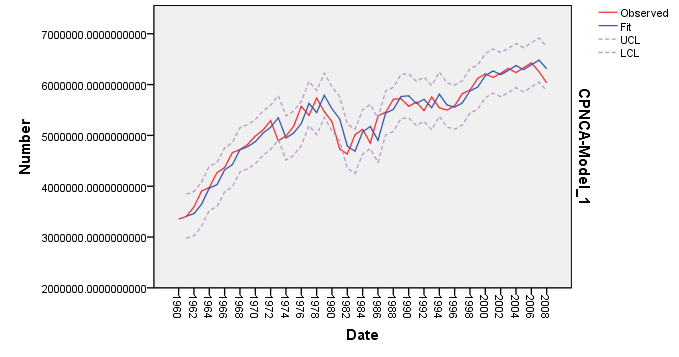
\includegraphics[width=0.6\textwidth]{./picture/CPNCA.png}}
  \caption{The evolution of CPN energy of CA}
\end{figure}

\begin{figure}[H]
  \centering{
  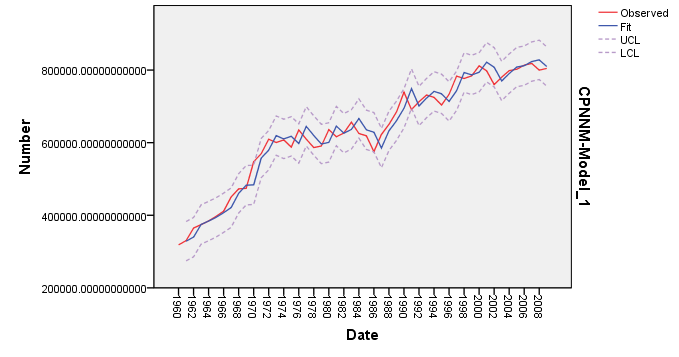
\includegraphics[width=0.6\textwidth]{./picture/CPNNM.png}}
  \caption{The evolution of CPN energy of NM}
\end{figure}

\begin{figure}[H]
  \centering{
  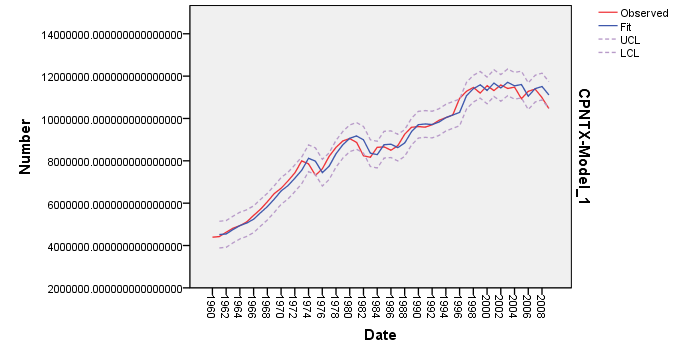
\includegraphics[width=0.65\textwidth]{./picture/CPNTX.png}}
  \caption{The evolution of CPN energy of TX}
\end{figure}

\section{Codes}

Here are programmes used for ARIMA model.\\

\textbf{\textcolor[rgb]{0.98,0.00,0.00}{Input matlab source:}}
\lstinputlisting[language=Matlab]{./code/time_series.m}

\end{appendices}
\end{document}
